\section{Bridging Looplets and Finch: The Tensor Interface}
%
%The Finch language provides descriptions of computations that iterate over a subset of a regular grid that is lexicographically ordered.
%
%Based on our description of Looplets, the reader might believe that compilation of a Finch program simply involves simply replacing for loops over a range with for loops over iterators.
%
%However, Finch's data structures and control flow are sufficiently complex that several challenges exist.
%
Arrays use multiple dimensions to organize data with respect to orthogonal concepts.
%
Thus, the Finch language supports multi-dimensional arrays.
%
Unfortunately, the Looplet abstraction is best suited towards iterators over a single dimension.
%
Our level abstraction provides a bridge between the single dimensional iterators created from looplets and the mutli-dimensional abstractions common to tensor compilers.
% 
This bridge must address three challenges.
%
First, looplets represent an instance of an iterator over a tensor, but we may access the same tensor twice with different indices.
%
Thus, the $unfurl$ function creates separate looplet nests for each iterator.
%
Next, since Finch programs are not just single einsums, they may read and write to the same data at different times.
%
The $declare$, $freeze$, and $thaw$ functions provide machinery to manage transition between these states.
%
Finally, we must be able to write looplet nests that modify tensors, as well as reading them.
%
The $assemble$ function manages the allocation of new data in the tensor.

\begin{wrapfigure}{R}{0.5\linewidth}
    \centering
    \vspace{-8pt}
    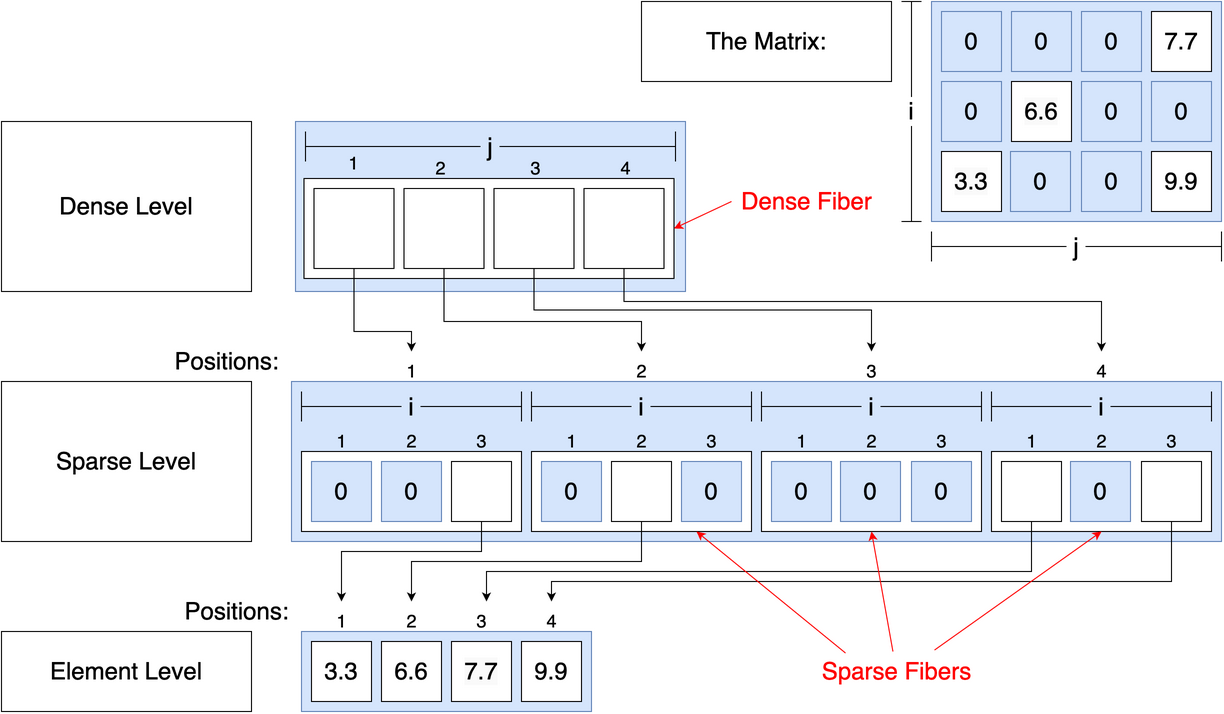
\includegraphics[width=\linewidth]{LevelsVsFibers-matrix.png}
    %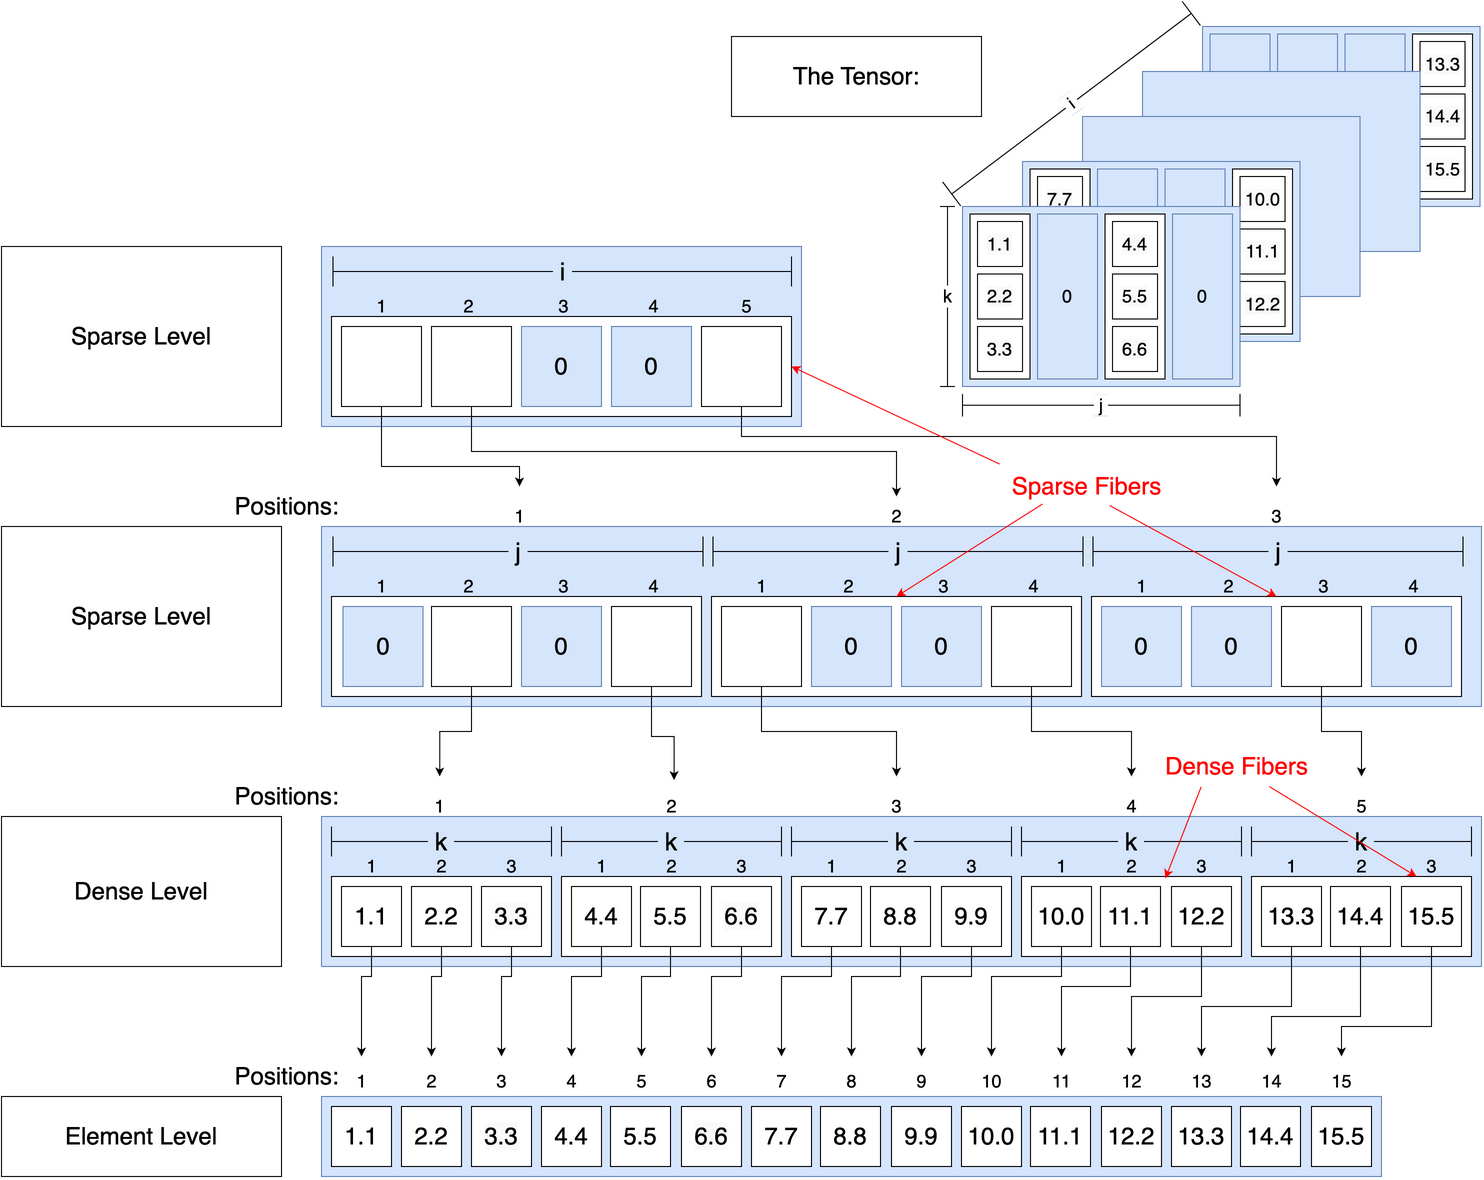
\includegraphics[width=0.5\linewidth]{LevelsVsFibers-tensor.png}
    \vspace{-8pt}
    \caption{Levels in the fiber tree representation of a sparse matrix in CSC format, with a dense outer level and a sparse inner level. The element level holds the leaves of the tree.}
    \label{fig:levelsvsfibers}
    \vspace{-8pt}
\end{wrapfigure}

In the rest of this section, we describe this functionality in detail after we review the basics of level abstractions~\cite{sze2017efficient,chou2022compilation, chou2018format}.
%
Then we discuss $declare$, $freeze$, $thaw$, and $unfurl$ functions as part of a life cycle abstraction as well as the $assemble$ function.
%
These interfaces add to the level abstraction, expanding the types of data that they can express via mapping to Looplets and expanding the contexts in which they can be used.
%
Finally, we describe several levels that we implement in this abstraction, which allow us to implement a taxonomy of known structures that appear in tensor computations.

% Previous efforts to compile a greater variety of sparse array programs left these bridges untouched ~\cite{henry_compilation_2021, won2023unified, senanayake2020sparse}

% \willow{After making changes to the introduction of this section, some of the following text feels redundant}
% To build our bridge, we embrace a set of abstractions: level formats/Fiber Trees, iteration context dependent instantiation of iterators, and tensor life cycles.
% %
% Our first abstraction mostly already exists in the literature: a manner of specifying a data structure for a multi-dimensional tensor out of data structures for single dimensional tensors
% %
% We recapitulate the essential details here.
% %
% Our next two abstractions add to to the first by providing a mechanism to use data structures generated by the first abstraction in a greater variety of contexts while maintaining per-dimension encapsulation of array data structures.
% %
% We introduce an interface to instatiate iterators in a variety of contexts in our programs and we introduce the lifecycle interface to manage when we read and write to multi-dimensional iterators.
% %
% These interfaces add to the level abstraction, expanding the types of data that they can express via mapping to looplets and expanding the contexts in which they can be used.
% %
% Previous efforts to compile a greater variety of sparse array programs left these bridges untouched ~\cite{henry_compilation_2021, won2023unified, senanayake2020sparse}.

%What needs to be said about the tensors? It's basically a few main points:
%1. (DONE) What is the level abstraction 
%2. (Done) We have identified 8 key level structures to represent most combinations of runs or pinpoints.
%2. (Done) a. beautiful figure with datas as rows of larger structures
%2. b. How do we write to each of these, in order? Randomly? random access? several important datastructures that show up along the way.
%3. What is "Unfurling"? and how does it help us represent each structure? refer to looplet decompositions of each case in the earlier figure
%4. (Done) What are lifecycles? How do lifecycles help us keep sane? Why are they necessary for correctness?

\subsection{Level Abstraction}

Fiber-tree style tensor abstractions have been the subject of extensive study
\cite{sze2017efficient, chou2022compilation, chou2018format}.  The underlying
idea is to represent a multi-dimensional tensor as a nested vector
datastructure, where each level of the nesting corresponds to a dimension of the
tensor. Thus, a matrix would be represented as a vector of vectors. This kind of
abstraction lends itself to representing sparse tensors if we vary the type of
vector used at each level in a tree. Thus, a sparse matrix might be represented
as a dense vector of sparse vectors. The vector of subtensors in this
abstraction is referred to as a \textbf{fiber}. Prior fiber-tree representations
focus on sparsity (where only the nonzero elements are represented) and treat
sparse vectors as sets of represented points. Since our fiber-tree
represesentation must handle other kinds of structure, such as diagonal,
repeated, or constant values, we instead view each fiber as a mapping from
indices into a space of subfibers.

%From the docs:
%Finch represents tensors hierarchically in a tree, where each node in the tree is a vector of subtensors and the leaves are the elements. Thus, a matrix is analogous to a vector of vectors, and a 3-tensor is analogous to a vector of vectors of vectors. The vectors at each level of the tensor all have the same structure, which can be selected by the user.
%In a Finch tensor tree, the child of each node is selected by an array index. All of the children at the same level will use the same format and share the same storage. Finch is column major, so in an expression A[i_1, ..., i_N], the rightmost dimension i_N corresponds to the root level of the tree, and the leftmost dimension i_1 corresponds to the leaf level.
%We refer to a node in the tree as a subfiber. All of the nodes at the same level are stored in the same datastructure, and disambiguated by an integer position. in the above example, there are three levels: the rootmost level contains only one subfiber, the root. The middle level has 3 subfibers, one for each column. The leafmost level has 12 subfibers, one for each element of the array. For example, the first level is A_fbr.lvl, and we can represent it's third position as SubFiber(A_fbr.lvl.lvl, 3). The second level is A_fbr.lvl.lvl, and we can access it's 9th position as SubFiber(A_fbr.lvl.lvl.lvl, 9). For instructional purposes, you can use parentheses to call a subfiber on an index to select among children of a subfiber.
%When we print the tree in text, positions are numbered from top to bottom. However, if we visualize our tree with the root at the top, positions range from left to right:
%Dense Format Index Tree
%Because our array is sparse, (mostly zero, or another fill value), it would be more efficient to store only the nonzero values. In Finch, each level is represented with a different format. A sparse level only stores non-fill values. This time, we'll use a tensor constructor with sl (for "SparseList of nonzeros") instead of d (for "Dense"):
%CSC Format Index Tree
%Our Dense(SparseList(Element(0.0))) format is also known as "CSC" and is equivalent to SparseMatrixCSC. The Tensor function will perform a zero-cost copy between Finch fibers and sparse matrices, when available. CSC is an excellent general-purpose representation when we expect most of the columns to have a few nonzeros. However, when most of the columns are entirely fill (a situation known as hypersparsity), it is better to compress the root level as well:
%DCSC Format Index Tree
%Here we see that the entirely zero column has also been compressed. The SparseList(SparseList(Element(0.0))) format is also known as "DCSC".
%The COO format is compact and straightforward, but doesn't support random access. For random access, one should use the SparseHash format. A full listing of supported formats is described after a rough description of shared common internals of level, relating to types and storage.
%All levels have a postype, typically denoted as Tp in the constructors, used for internal pointer types but accessible by the function:
%postype(lvl)


Instead of storing the data for each subfiber separately, most sparse tensor
formats such as CSR, DCSR, and COO usually store the data for all fibers in a
level contiguously. In this way, we can think of a level as a bulk allocator for
fibers. Continuing the analogy, we can think of each fiber as being
disambiguated by a \textbf{position}, or an index into the bulk pool of
subfibers. The mapping $f$ from indices to subfibers is thus a mapping from an
index and a position in a level to a subposition in a sublevel.
Figure~\ref{fig:levelsvsfibers} shows a simple example of a level as a pool of fibers.

When we need to refer to a particular fiber at position $p$ in the level $l$, we
may write $fiber(l, p)$. Note that the formation of fibers from levels is lazy,
and the data underlying each fiber is managed entirely by the level, so the
level may choose to overlap the storage between different fibers. Thus, the only
unique data associated with $fiber(l, p)$ is the position $p$.

\subsection{Tensor Lifecycle, Declare, Freeze, Thaw, Unfurl}

Our simplified view of a level is enabled by our use of looplets to represent
the structure within each fiber.
%
In fact, our level interface requires only 5
highly general operations, described below.

The first three of these functions, declare, freeze, and thaw, \saman{Italics for keywords?}have to do with
managing when tensors can be assumed mutable or immutable.
%
\saman{This is because Finch goes beyond just a single einsum...the scope of Finch w.r.t. TACO etc, is not clear.}
%
As we use Looplets to
represent iteration over a tensor, we must restrict the mutability of tensors
while we iterate over them. 
%
For example, if a tensor declares it has a constant
region from $i = 2:5$, but some other part of the computation modifies the
tensor at $i = 3$, this would result in incorrect behavior.
%
It is much easier to
write correct Looplet code if we can assume that the tensor is immutable while
we are reading from it.
%
Thus, we introduce the notion that a tensor can be in
read-only mode or update-only mode.  
%
In read-only mode, the tensor may only
appear in the right-hand side of assignments
%
. In update-only mode, the tensor
may only appear in the left-hand side of an assignment, either being overwritten
or incremented by some operator. 
%
We can switch between these modes using freeze
and thaw functions.
%
The declare function is used to allocate a tensor,
initialize it to some specified size and value, and leave it in update-only
mode. 

The unfurl function is used to manage iteration over a subfiber. 
%
At the point when it comes time to iterate over a tensor, be in on the left or right hand
side of an assignment, we call the unfurl function to precompute whatever state
and datastructures are necessary to return a looplet nest that would iterate
over that level of a tensor.
%
The unfurl function is called directly before
iterating over the corresponding loop, so it has access to any state variables introduced
by freezing or thawing the tensor.

\begin{figure}[htbp]
    \scriptsize
    \raggedright
\fbox{\parbox{\textwidth}{$declare(lvl, init, dims...)$: Declares the level to hold subtensors of size $dims$ and an initial value of $init$. Requires the level to be in
read-only mode.}}

\vspace{3pt}

\fbox{\parbox{\textwidth}{$freeze(lvl)$: Finalizes the updates in the level, and readies the
level for reading. Requires the level to be in update-only mode.}}

\vspace{3pt}

\fbox{\parbox{\textwidth}{$thaw(lvl)$: Prepares the level to accept updates. Requires the level
to be in read-only mode.}}

\vspace{3pt}

\fbox{\parbox{\textwidth}{$unfurl(fiber(lvl, pos), [ext], mode, [op], [rhs])$: When $ext$ is given, unfurls the fiber at position
$pos$ in the level $lvl$ over the extent $ext$. When $mode = \finchread$,
returns a looplet nest over the values in the read-only fiber.  When $mode =
\finchupdate$, returns a looplet nest over mutable subfibers in the update-only
fiber. When applied to a scalar or leaf node, $ext$ is omitted and we may also use $op$ and $rhs$ to update the scalar value. Often, skipping over mutable locations allows the level to know which
locations must be stored. Often, a dirty bit may be used in $tns$ to communicate
whether the mutable subfiber has been written to, which allows the parent fiber
to know whether the subfiber must be stored explicitly.}}

\vspace{3pt}

\fbox{\parbox{\textwidth}{$assemble(lvl, pos_{start}, pos_{stop})$: Allocates subfibers in the
level from positions $pos_{start}$ to $pos_{stop}$. Usually, this function is
only ever called on unassembled positions, but some levels (such as dense levels
or bytemaps) may support reassembly.}}
\vspace{-8pt}
\caption{The five functions that define a level.}
\vspace{-12pt}
\end{figure}




\begin{figure}[ht]
\footnotesize
\begin{tabular} {|c|p{0.65\linewidth}|} 
    \hline
    $declare(lvl, init, dims...)$ & Declares the level to hold subtensors of size $dims$ and an initial value of $init$. Requires the level to be in
read-only mode.
\hline


    \end{tabular}


\vspace{3pt}

\fbox{\parbox{\textwidth}{$freeze(lvl)$: Finalizes the updates in the level, and readies the
level for reading. Requires the level to be in update-only mode.}}

\vspace{3pt}

\fbox{\parbox{\textwidth}{$thaw(lvl)$: Prepares the level to accept updates. Requires the level
to be in read-only mode.}}

\vspace{3pt}

\fbox{\parbox{\textwidth}{$unfurl(fiber(lvl, pos), [ext], mode, [op], [rhs])$: When $ext$ is given, unfurls the fiber at position
$pos$ in the level $lvl$ over the extent $ext$. When $mode = \finchread$,
returns a looplet nest over the values in the read-only fiber.  When $mode =
\finchupdate$, returns a looplet nest over mutable subfibers in the update-only
fiber. When applied to a scalar or leaf node, $ext$ is omitted and we may also use $op$ and $rhs$ to update the scalar value. Often, skipping over mutable locations allows the level to know which
locations must be stored. Often, a dirty bit may be used in $tns$ to communicate
whether the mutable subfiber has been written to, which allows the parent fiber
to know whether the subfiber must be stored explicitly.}}

\vspace{3pt}

\fbox{\parbox{\textwidth}{$assemble(lvl, pos_{start}, pos_{stop})$: Allocates subfibers in the
level from positions $pos_{start}$ to $pos_{stop}$. Usually, this function is
only ever called on unassembled positions, but some levels (such as dense levels
or bytemaps) may support reassembly.}}
\vspace{-8pt}
\caption{The five functions that define a level.}
\vspace{-12pt}
\end{figure}

% \begin{figure}[htbp]
%     \scriptsize
% \begin{tabular}{|p|p|} 
% \hline
%      Function & Description  \\
%      \hline
%      $declare(lvl, init, dims...)$ & Declares the level to hold subtensors
% of size $dims$ and an initial value of $init$. Requires the level to be in
% read-only mode.\\
% \hline
% $freeze(lvl)$ & Finalizes the updates in the level, and readies the
% level for reading. Requires the level to be in update-only mode.\\
% \hline
% $thaw(lvl)$ & Prepares the level to accept updates. Requires the level
% to be in read-only mode.\\
% \hline
% $unfurl(fiber(lvl, pos), [ext], mode, [op], [rhs])$ & When $ext$ is given, unfurls the fiber at position $pos$ in the level $lvl$ over the extent $ext$. When $mode = \finchread$, returns a looplet nest over the values in the read-only fiber.  When $mode = \finchupdate$, returns a looplet nest over mutable subfibers in the update-only fiber. When applied to a scalar or leaf node, $ext$ is omitted and we may also use $op$ and $rhs$ to update the scalar value. Often, skipping over mutable locations allows the level to know which
% locations must be stored. Often, a dirty bit may be used in $tns$ to communicate
% whether the mutable subfiber has been written to, which allows the parent fiber
% to know whether the subfiber must be stored explicitly.\\
% \hline


% \end{tabular}
% \caption{The five functions that define a level.}
% \vspace{-12pt}
% \end{figure}


Our view of a level as a fiber allocator implies an allocation function
$assemble(tns, pos_{start}:pos_{stop})$, which allocates fibers at positions
$pos_{start}:pos_{stop}$ in the level. We don't specify a de-allocation
function, instead relying on initialization to reset the fiber if it needs to be
reused. While all of the previous functions are used to manage the lifecycle and
iteration over a general tensor, the assemble function is quite specific to the
level abstraction, and the notion of positions within sublevels. Note: it was an
intentional choice to hold the parent level responsible for managing the
data of the sublevels, which positions they allocate, etc. This allows the parent
level to reuse allocation logic from internal index datastructures. For example,
a sparse level might use a list of indices to store which nonzeros are present,
and when it comes time to resize that list, it could also call assemble to resize the
sublevel, reducing the number of branches in the code. The assemble function
lends itself particularly to a "vector doubling" allocation approach, which we
have found to be effective and flexible when managing the allocation
of sparse left hand sides. This benefit is made clear in our evaluation section,
where we see that prior systems like TACO do not support all possible loop
orderings and format combinations for sparse matrix multiply because they do
not have a flexible enough allocation strategy, instead using a two-phase approach
which requires computing a complicated closed-form kernel to iterate over the
data twice to determine the number of required output nonzeros.

\subsection{The 8 Key Level Structures}

    The main benefits of specializing to structure come from the following properties of the data:
    \begin{itemize}
        \item \textbf{Sparsity} Sparse data is data that is mostly zero, or some other
        fill value. When we specialize on this data, we can use annihilation ($x
        * 0 = 0$), identity ($x * 1 = 1$), or other constant propagation
        properties ($ifelse(false, x, y) = y$) to simplify the computation and avoid
        redundant work.
        
        \item \textbf{Blocks} Blocked data is a subset of sparse data where the nonzeros
        are clustered and occur adjacent to one another. This provides us with
        two opportunities: We can avoid storing the locations of the nonzeros
        individually, and we can use more efficient randomly accessible
        iterators within the block. \cite{im_optimizing_2001, vuduc_performance_2002, ahrens_looplets_2023}.

        \item \textbf{Runs} Runs of repeated values may occur in dense or sparse code,
        cutting down on storage and allowing us to use integration rules such as 
        \mintinline{julia}{for i = 1:n; s += x end} $\rightarrow$
        \mintinline{julia}{s += n * x} or code motion to lift operations out of loops \cite{donenfeld_unified_2022,ahrens_looplets_2023}.

        \item \textbf{Singletons} When we have only one non-fill region in sparse data,
        we can avoid a loop entirely and reduce the complexity of iteration \cite{ghorbani2023compiling, ahrens_looplets_2023}.
    \end{itemize}

   We consider all combinations of these structural properties in Table
    \ref{tab:TypesOfStructure}, resulting in 8 key level formats that correspond
    the the 8 resulting situations. While it is impossible to write code which
    precisely addresses every possible structure, the combination of our level
    formats can express a wide variety of hierarchical structures to a
    sufficient granularity that we can generate code which utilizes the four
    properties.  For example, though banded arrays are a superset of ragged
    arrays, representing a ragged array using a banded format does not add much
    overhead.  The structures we consider are exhaustive in the sense that they
    address all combinations of sparsity, blocks, runs, and singletons in each
    level. We can represent a wide variety of hierarchical tensor structures by
    combining these level structures in a tree, as shown in
    Figure~\ref{fig:structuraldiversity}.

    \begin{wrapfigure}{r}{.35\textwidth}
        \centering
        \vspace{-8pt}
        \scriptsize
        \begin{tabular}{|c|c|c|c|l|}
            \hline
            \rothead{Sparse} & \rothead{Blocked} & \rothead{Runs} & \rothead{Singletons} & \begin{tabular}{@{}l@{}}\textbf{Corresponding} \\ \textbf{Format}\end{tabular} \\
            \hline
             &  &  &  & Dense \\
            \hline
             &  & \checkmark &  & DenseRLE \\
            \hline
            \checkmark &  &  &  & Sparse \\
            \hline
            \checkmark &  &  & \checkmark & SparsePinpoint \\
            \hline
            \checkmark &  & \checkmark &  & SparseRLE \\
            \hline
            \checkmark &  & \checkmark & \checkmark & SparseInterval \\
            \hline
            \checkmark & \checkmark &  &  & SparseVBL \\
            \hline
            \checkmark & \checkmark &  & \checkmark & SparseBand \\
            \hline
        \end{tabular}
        \vspace{-8pt}
        \caption{All combinations of relevant structural properties and their
        corresponding formats.  Note that blocks and runs need not be considered
        together because we must store a run length for each run, and so there
        isn't a significant storage benefit to combining them. Blocks and
        singletons only make sense in the contex of sparsity, so we don't
        consider them together either. We omit such combinations
        from the exhaustive table.}
        \label{tab:TypesOfStructure}
        \vspace{-12pt}
    \end{wrapfigure}

 
    
    \begin{figure}
        \centering
        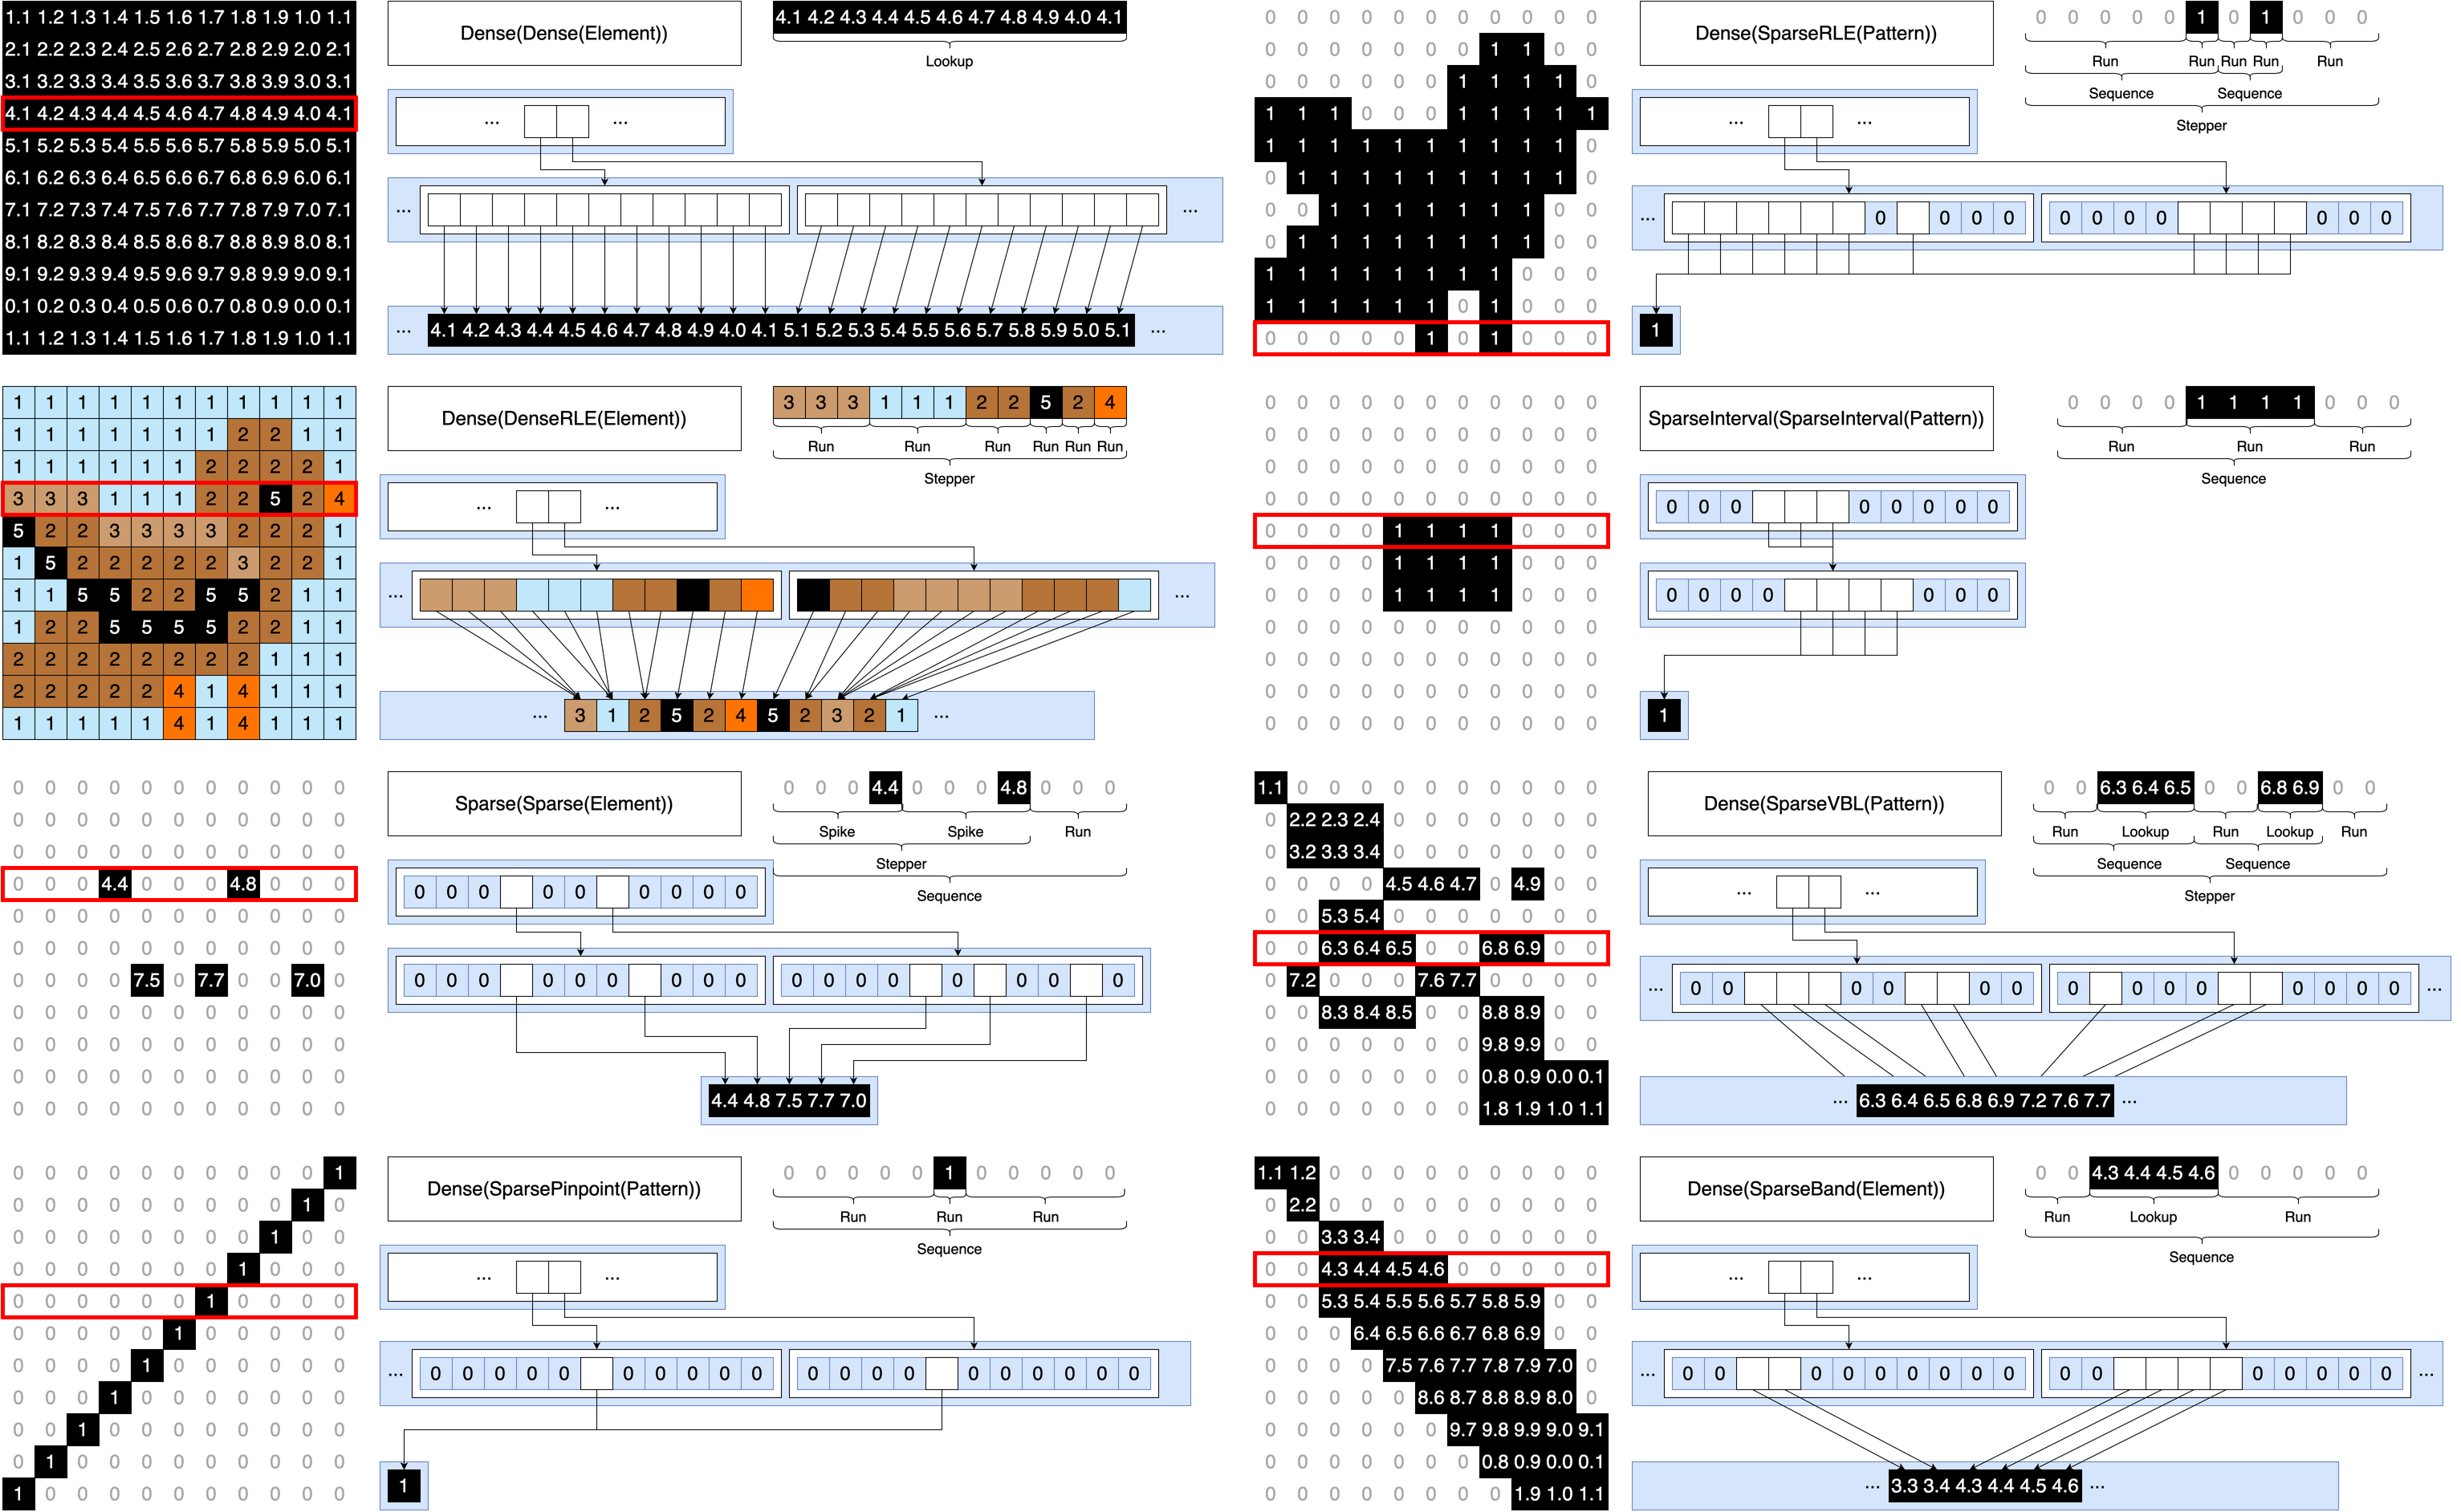
\includegraphics[width=\linewidth]{Structures.png}\hfill%
        \vspace{-8pt}
        \caption{Several examples of matrix structures represented using the
        level structures identified in Table~\ref{tab:TypesOfStructure}.
        Comparing this figure to \cite[Figure 3]{ahrens_looplets_2023}, we see
        that a level-by-level structural decomposition is diagrammed together
        with the Looplets.}
        \label{fig:structuraldiversity}
        \vspace{-18pt}
    \end{figure}

\subsection{Randomly Accessible Temporary Levels}
To reduce the implementation burden and improve efficiency in the common case, the levels we described in the previous section only support bulk,
sequential creation of formats. However, when users want to be able to write out
of order (which is a common requirement arising from loop order or from the
problem itself, it occurs in our spgemm algorithms and our histogram example in
the evaluation section), we must use more complicated datastructures like hash
tables and trees to support the random access. Because these datastructures are
more complex and have a higher implementation burden and performance overhead,
we only support random access construction of sparse or dense structures.  We
can use these two more general structures as intermediates to convert to our
more specialized structures later.

\HIDE{\saman{Can we not put future work into the submission!} As future work, we also recommend the implementation of a tree-based format, as this would enable incremental construction. Currently, the cost of freezing and thawing is usually proportional to the number of stored fibers, so an operation that sets a single value in a tensor would be prohibitively expensive (i.e.  $A[3, 4] = 3.14$). We would also recommend supporting SparseRLE as an intermediate randomly accessible structure, because (unlike blocks or singletons), runs have asymptotic benefits. However, these cases were not necessary for our case studies.}

\help{this section fails to address freeze or thaw and how it relates to the concrete levels}

\subsection{Leaf Levels}

The leaf level stores the actual entries of the tensor. In most cases, it is
sufficient to store each entry at a separate position in a vector. This is accomplished by the \textbf{ElementLevel}. However, when all of the
values are the same, an additional optimization can be made by storing the
identical value only once. In this work, we introduce the concept of a \textbf{pattern}
level to handle this binary case. Pattern has a fill value of $false$, and returning $true$ for all ``stored'' values. The pattern level allows us to easily represent unweighted graphs or other boolean matrices.

\subsection{Scalars}
Because elements are geared towards representing many leaves in a level, we also introduce a much simpler Scalar format to represent 0-dimensional tensors.
%
Scalars can also affect how the leaves are lowered.
%
Constant propagation through arrays is known to be a complex compiler pass \cite{mcmichen_representing_nodate}.
%
Instead, we provide sparse scalars, which allow reductions but also specialize read accesses for the possible zero value.
%
We also provide early break scalars, which modify the stepper looplets to
re-specialize the loop whenever a reduction into an early break scalar hits an
annihilator.
%
We assume that we don't need to re-specialize other looplets because the stepper
is the only one which repeats a non-constant number of times.

\begin{table}[ht]
    \centering
    \scriptsize
    \renewcommand{\arraystretch}{1.3}
    \begin{tabular}{p{14cm}}

    \hline
    \textbf{Sequential Access Levels} \\
    \hline
    \textbf{Dense}:
    The dense format is the simplest format, mapping $fiber(l, p)[i] \rightarrow fiber(l.lvl, p \times l.shape + i)$.
    %
    This format is used to store dense data and is often a convenient format for the root level of a tensor.
    %
    Due to its simplicity, freezing and thawing the level are no-ops. \\
    \textbf{DenseRLE}:
    Used to represent runs of repeated values, storing two vectors, $right$ and $ptr$, with $qth$ run in the $p^th$ subfiber starting and ending at $right[ptr[p] + q]$ and $right[ptr[p] + q + 1] - 1$, respectively.
    %
    A challenge arises for this level: it is difficult to merge duplicate runs.
    %
    Such a scenario might arise when merging runs of subfibers of length 3, representing colors in an image.
    %
    Ideally, we would be able to detect duplicate subfibers and merge them on the fly, but we cannot determine which subfibers are equal because we cannot read them while the sublevel is in update-only mode.
    %
    Instead, we merge the duplicates during the freeze phase.
    %
    We $freeze$ the sublevel, $declare$ a separate sublevel $buf$ as a buffer to store the deduplicated subfibers, and then compare each of the subfibers in the main level, copying the deduplicated subfibers into the buffer. \\
    %
    %It also stores a duplicate sublevel, $buf$, for deduplication. \\
    \textbf{SparseList}:
    The simplest sparse format, used to construct popular formats like CSR, CSC, DCSR, DCSC, and CSF.
    %
    It stores two vectors, $idx$ and $ptr$, such that $idx[ptr[p] + q]$ is the index of the $qth$ nonzero in the subfiber at position $p$. \\
    \textbf{SparsePinpoint}:
    Similar to SparseList, but only one nonzero in each subfiber, eliminating the need for the $ptr$ field.
    %
    It stores a vector $idx$, such that $idx[p]$ is the nonzero index in the subfiber at position $p$. \\
    \textbf{SparseRLE}:
    Similar to DenseRLE level, but because runs are sparse, we must also store the start of each run.
    %
    It stores three vectors $left$, $right$, and $ptr$, such that the $qth$ run in the $p^th$ subfiber begins and ends at $left[ptr[p] + q]$ and $right[ptr[p] + q]$, respectively.
    %
    Like DenseRLE, it also stores a duplicate sublevel, $buf$, for deduplication. \\
    \textbf{SparseInterval}:
    Similar to SparseRLE, but only stores one run per subfiber, eliminating the need for the $ptr$ field.
    %
    This level does not deduplicate as it cannot store intermediate results with more than one run.
    %
    It stores two vectors, such that the run in subfiber $p$ begins and ends at $left[p]$ and $right[p]$ respectively. \\
    \textbf{SparseVBL}: Used to represent blocked data. It stores three vectors, $idx$, $ptr$, and $ofs$, such that $ofs[ptr[p] + q]:ofs[ptr[p] + q + 1] - 1$ are the subpositions of block $q$ ending at index $idx[ptr[p] + q]$ in the subfiber at position $p$. \\
    \textbf{SparseBand}: Similar to SparseVBL, but stores only one block per subfiber, eliminating the need for the $ptr$ field. It stores two vectors $idx$ and $ofs$, such that $ofs[p]:ofs[p + 1] - 1$ are the subpositions of the block ending at $idx[p]$ in subfiber $p$. \\

    \hline
    \textbf{Random Access Levels} \\
    \hline
    \textbf{SparseHash}:
    The sparse hash format uses a hash table to store the locations of nonzeros, and sorts the unique indices for iteration during the freeze phase.
    %
    This allows for efficient random access, but not incremental construction, as the freeze phase runs in time proportional to the number of nonzeros in the entire level.
    %
    It stores two vectors, $idx$ and $ptr$, such that $idx[ptr[p] + q]$ is the index of the $qth$ nonzero in the subfiber at position $p$. 
    %
    Also stores a hash table $tbl$ for construction and random access in the level. \\
    \textbf{SparseBytemap}
    The SparseBytemap format uses a bytemap to store which locations have been written to.
    %
    Unlike the SparseHash format, the bytemap assembles the entire space of possible subfibers.
    %
    This accelerates random access in the format, but requires a high memory overhead.
    %
    Because we don't want to reallocate all of the memory in each iteration, the declaration of this format instead re-assembles only the dirty locations in the tensor.
    %
    This format is analogous to the default workspace format used by TACO.
    %
    It stores two vectors, $idx$ and $ptr$, such that $idx[ptr[p] + q]$ is the index of the $qth$ nonzero in the subfiber at position $p$.
    %
    These vectors are used to collect dirty locations.
    %
    It also stores $tbl$, a dense array of booleans such that $tbl[shape * p + i]$ is true when there is a nonzero at index $i$ in the subfiber at position $p$. \\
    \hline
    \textbf{Leaf Levels} \\
    \hline
    \textbf{Element}:
    The element level uses an array $val$ to store a value for each position $p$. The zero (fill) value is configurable.\\
    \textbf{Pattern}:
    The pattern level statically represents a leaf level with a fill value of $false$ and whose stored values are all $true$. \\
    \hline
    \textbf{Scalars} \\
    \hline
    \textbf{Scalar}:
    A dense scalar that, unlike a variable, supports reduction.  \\
    \textbf{SparseScalar}:
    A scalar with a dirty bit which specializes on the fill value when it occurs.\\
    \textbf{EarlyBreakScalar}:
    A scalar which triggers early breaks in reductions whenever an annihilator is encountered.\\
    \hline
    \end{tabular}
    \caption{The main level formats supported by Finch. Note that all non-leaf
    levels store a the dimension of the subfibers and a child level. Since we
    must be able to handle the case where a sublevel is not stored because a
    parent level is sparse, all of Finch's sparse formats use a dirty bit during
    writing to determine whether the sublevel has been modified from it's
    default fill value and thus, whether it needs to be stored.}
    \label{table:formats}
\end{table}
